\documentclass{article}
\usepackage{graphicx} % For including images
\usepackage{titling}  % For custom title page
\usepackage{circuitikz}
\usepackage{amsmath}
\usepackage{amssymb}
\usepackage{booktabs,tabu}
\usepackage[all, cmtip]{xy}
\newcommand{\ohm}{\Omega}
% Set up title and author
\title{Experiment 1: Basic Filter Design}
\author{Samyak Sheersh,Souhardya Bose,Aryam Shankar}
\date{27 August 2024}
\newcommand{\subtitle}[1]{%
  \posttitle{%
    \par\end{center}
    \begin{center}\large#1\end{center}
    \vskip0.5em}%
}

\begin{document}

% Custom title page
\begin{titlepage}
    \centering
    
\includegraphics[width=0.2\textwidth]{KGP_logo.png}\par\vspace{1cm}
    {\scshape\LARGE Department of Electronics and Electrical Communication Engineering, IIT Kharagpur\par}
    \vspace{1cm}
    {\huge\bfseries Experiment 3: AM Modulation using IC MC 1496\par}
    \vspace{1.5cm}
    {\Large\itshape Samyak Sheersh, Souhardya Bose, Aryam Shankar\par}
    \vfill
    % Identifying information at the bottom
    {\large Roll Numbers: 22EC30045, 21EE10097, 22EC3FP37\par}
    {\large Group Number: 12\par}
    \vfill
    {\large 27 August 2024\par}
\end{titlepage}



\section{Objectives}
\begin{figure}[!ht]
  \caption{Circuit Diagram}
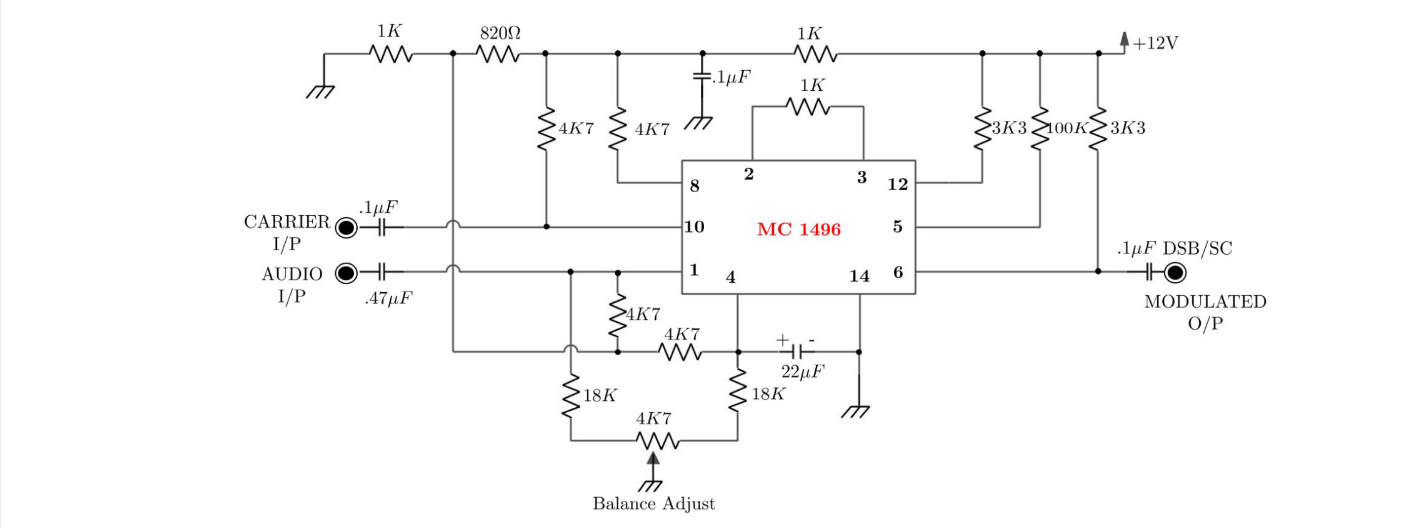
\includegraphics[width=\textwidth]{Circuit_diagram.png}
\end{figure}
\begin{enumerate}
  \item Make connections as in Figure 1 for an AM Modulator
  \item Set the carrier input signal as a sine wave with $A_c=300\ mV_{pp}$ and $f_c=20kHz$, and the message signal as a sine wave with $A_m=150mV_{pp}$ and $f_c=2kHz$
  \begin{equation}
      \Rightarrow m(t)=150\sin\left(2\pi\cdot 2\cdot 10^{3}\cdot t\right)
  \end{equation}
  \begin{equation}
      \Rightarrow c(t)=300\sin\left(2\pi\cdot 20\cdot 10^{3}\cdot t\right)
  \end{equation}
  \item Observe the modulated output at (Pin No. 6) and adjust the potentiometer (VR - Balance Adjust) so that the signal at AM o/p is maximum without distortion.
  \item Calculate the Modulation Index($m=\frac{A_m}{A_c}$)
    \begin{equation}
      m=\frac{A_{max}-A_{min}}{A_{max}+A_{min}}
    \end{equation}
  \item Observe the modulated o/p signal in frequency domain, and find $f_c$, $f_c+f_m$ and $f_c-f_m$.
  \item By varying the amplitude of the message signal($A_m$), observe the under-modulated, critically modulated, and over-modulated o/p waveforms in both time and frequency domain.
  \item Adjust the potentiometer (VR) to suppress the carrier signal in the Modulated output and observe the double side band suppressed carrier output. Also observe the o/p signal in frequency domain.
\end{enumerate}
\section{Instruments and Materials Used}
\begin{enumerate}
  \item RIGOL Signal Generator
  \item ScientiFIC SMO10C Digital Signal Oscilloscope
  \item +12V, -12V DC source and ground
  \item MC 1496 integrated circuit
  \item Resistors
  \item Capacitors
  \item Diodes
  \item Breadboard
  \item Connecting wires
\end{enumerate}

\section{Observations}
\subsection{Undermodulation}
$A_m=150\ mV_{pp}$: $A_{max}=176 \ mV_{pp}$, $A_{min}=64\ mV_{pp}$
\begin{equation}
  m_{U}=\frac{A_{max}-A_{min}}{A_{max}+A_{min}}=\frac{176-64}{176+64}=\frac{112}{240}=0.4667
\end{equation}
\begin{figure}[!ht]
  \caption{Undermodulated o/p waveform}
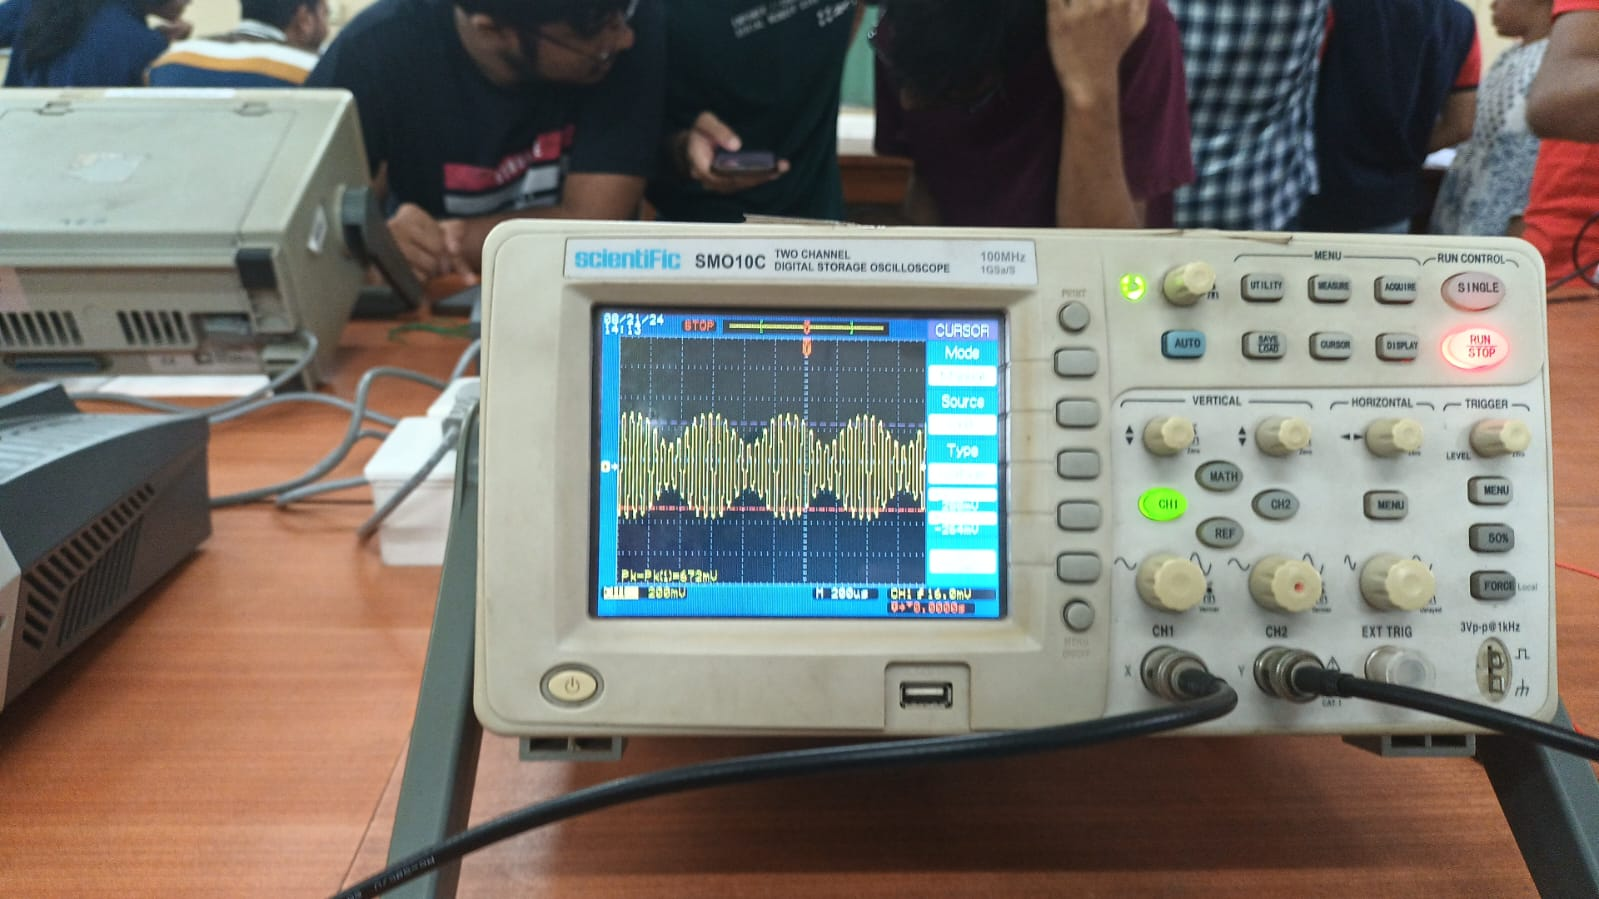
\includegraphics[width=\textwidth]{Undermodulation.jpeg}
\label{fig:Undermodulation}
\end{figure}
\begin{figure}[!ht]
  \caption{FFT of the Undermodulated o/p waveform}
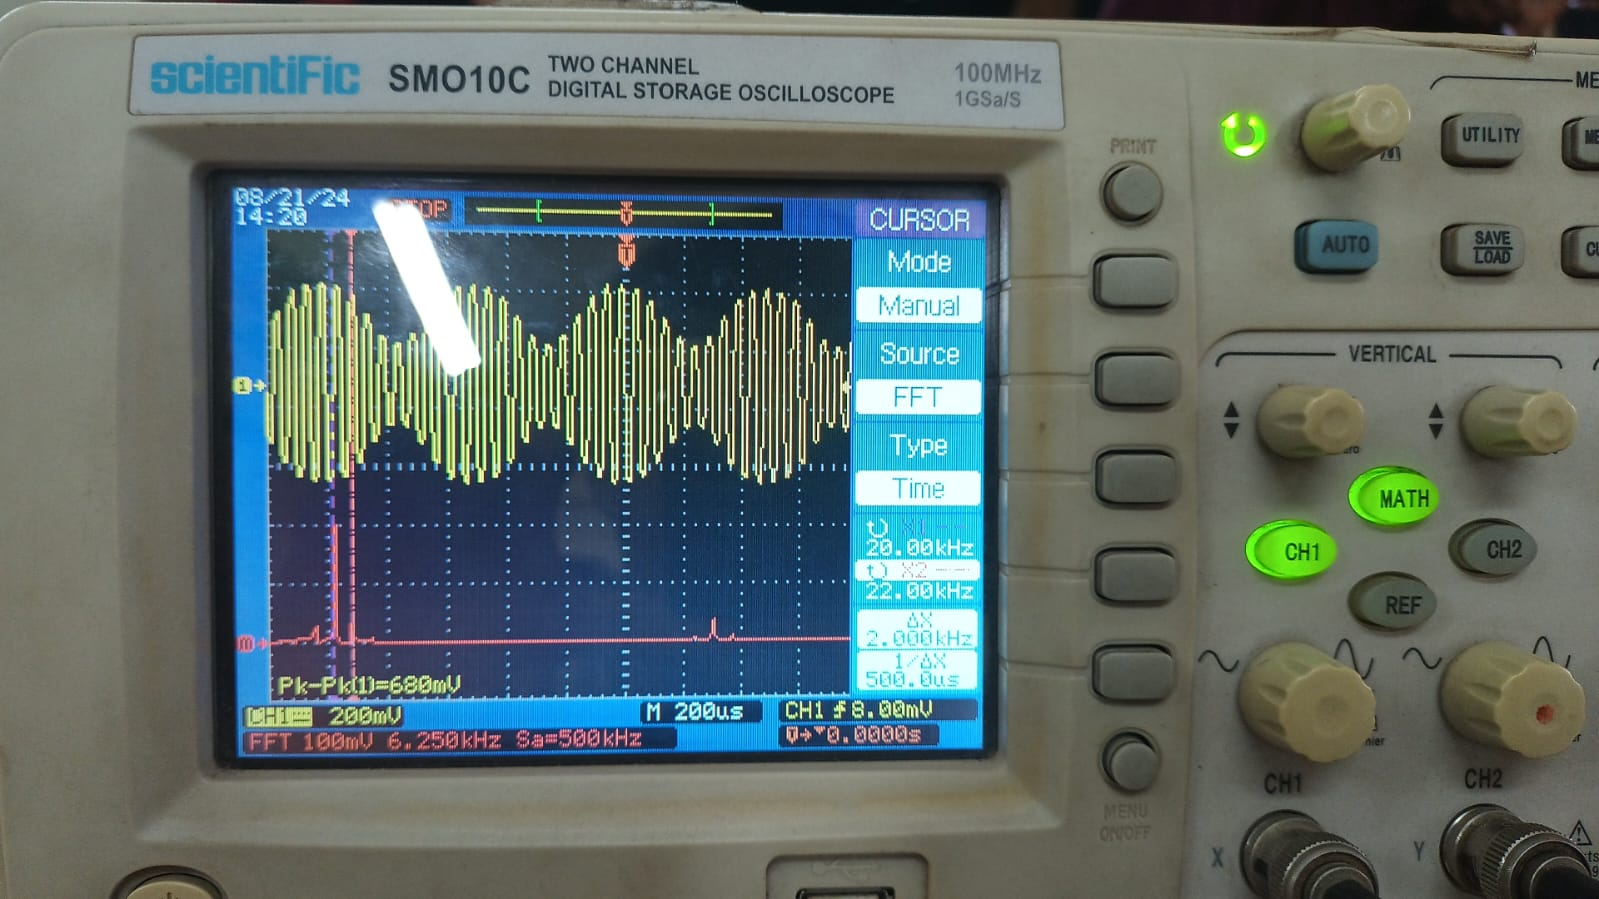
\includegraphics[width=\textwidth]{Undermodulation_FFT.jpeg}
\label{fig:Undermodulation_FFT}
\end{figure}
We see a peak at 20kHz, and 2 much smaller peaks at 18 and 22kHz
\clearpage
\subsection{Critical Modulation}
$A_m=300\ mV_{pp}$: $A_{max}=176 \ mV_{pp}$, $A_{min}=4\ mV_{pp}$
\begin{equation}
  m_{C}=\frac{A_{max}-A_{min}}{A_{max}+A_{min}}=\frac{176-4}{176+4}=\frac{172}{180}=0.955
\end{equation}
\begin{figure}[!ht]
  \caption{Critically modulated o/p waveform}
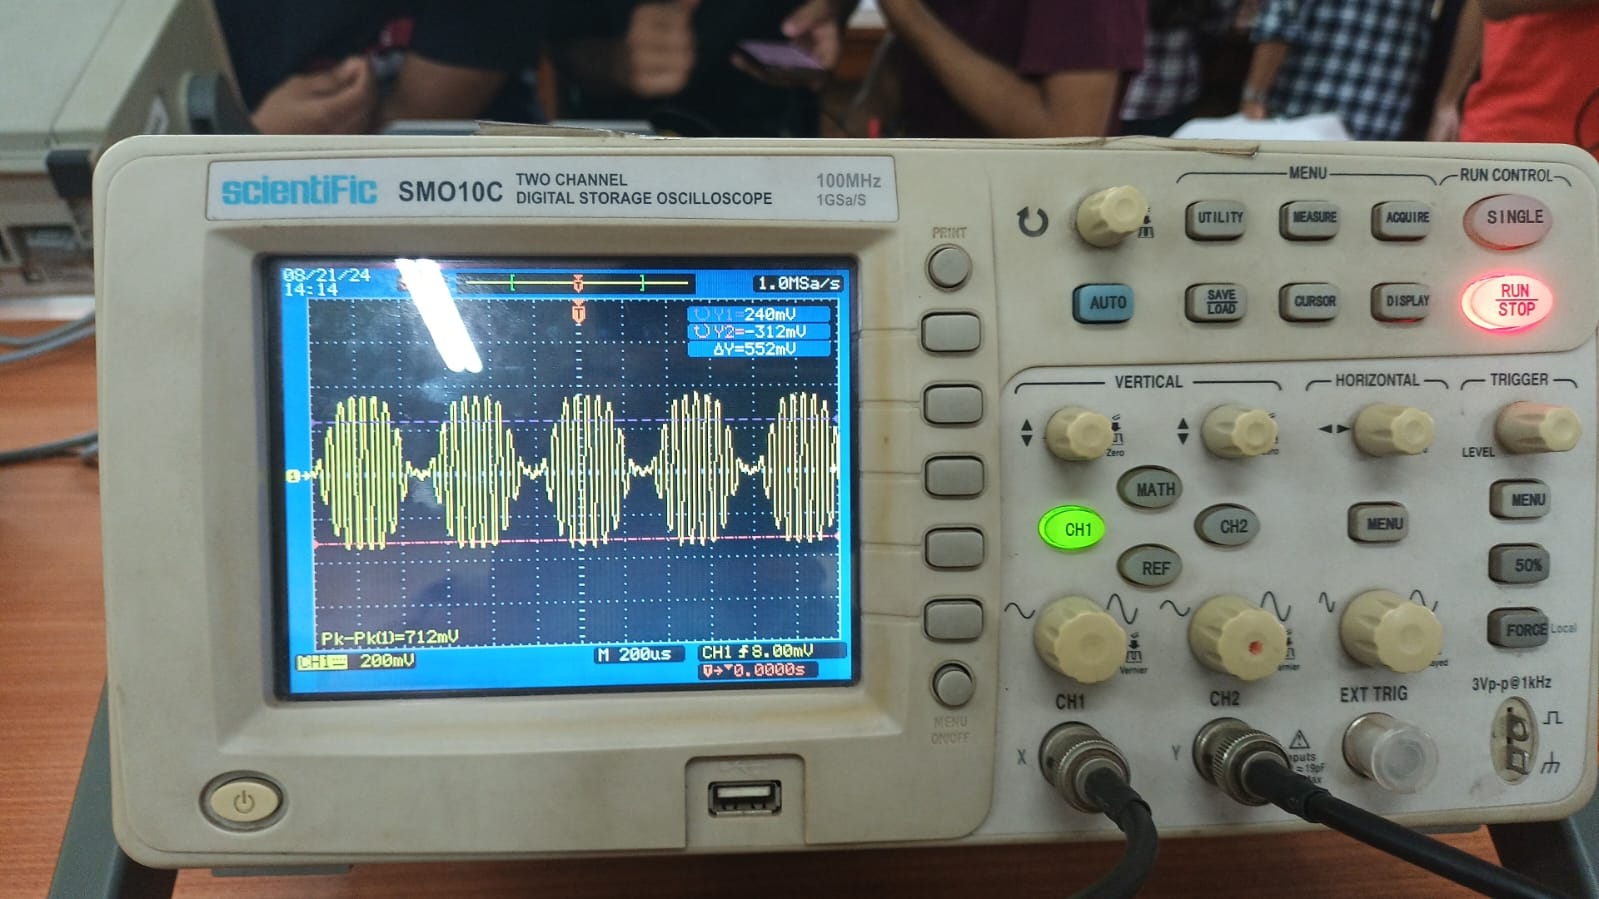
\includegraphics[width=\textwidth]{Critical_Modulation.jpeg}
\label{fig:Critical_modulation}
\end{figure}

\begin{figure}[!ht]
  \caption{FFT of the critically modulated o/p waveform}
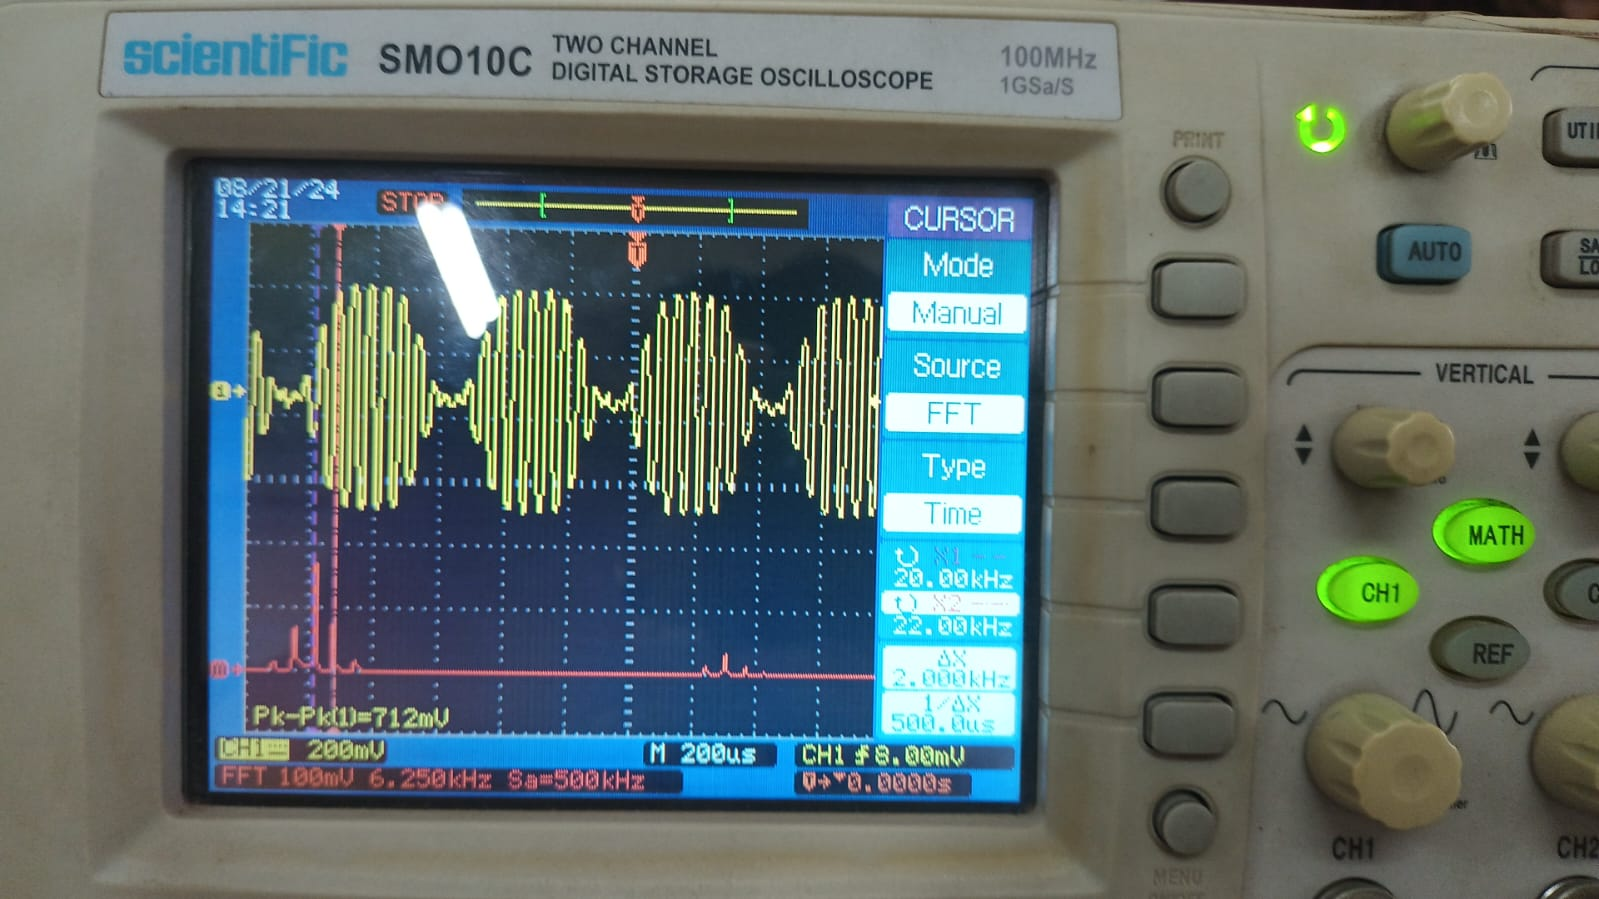
\includegraphics[width=\textwidth]{Critical_Modulation_FFT.jpeg}
\label{fig:Critical_modulation_FFT}
\end{figure}
\clearpage
\subsection{Overmodulation}
$A_m=400\ mV_{pp}$: $A_{max}=176 \ mV_{pp}$, $A_{min}=-48\ mV_{pp}$
\begin{equation}
  m_{O}=\frac{A_{max}-A_{min}}{A_{max}+A_{min}}=\frac{176+48}{176-48}=\frac{224}{128}=1.75
\end{equation}
\begin{figure}[!ht]
  \caption{Overmodulated o/p waveform}
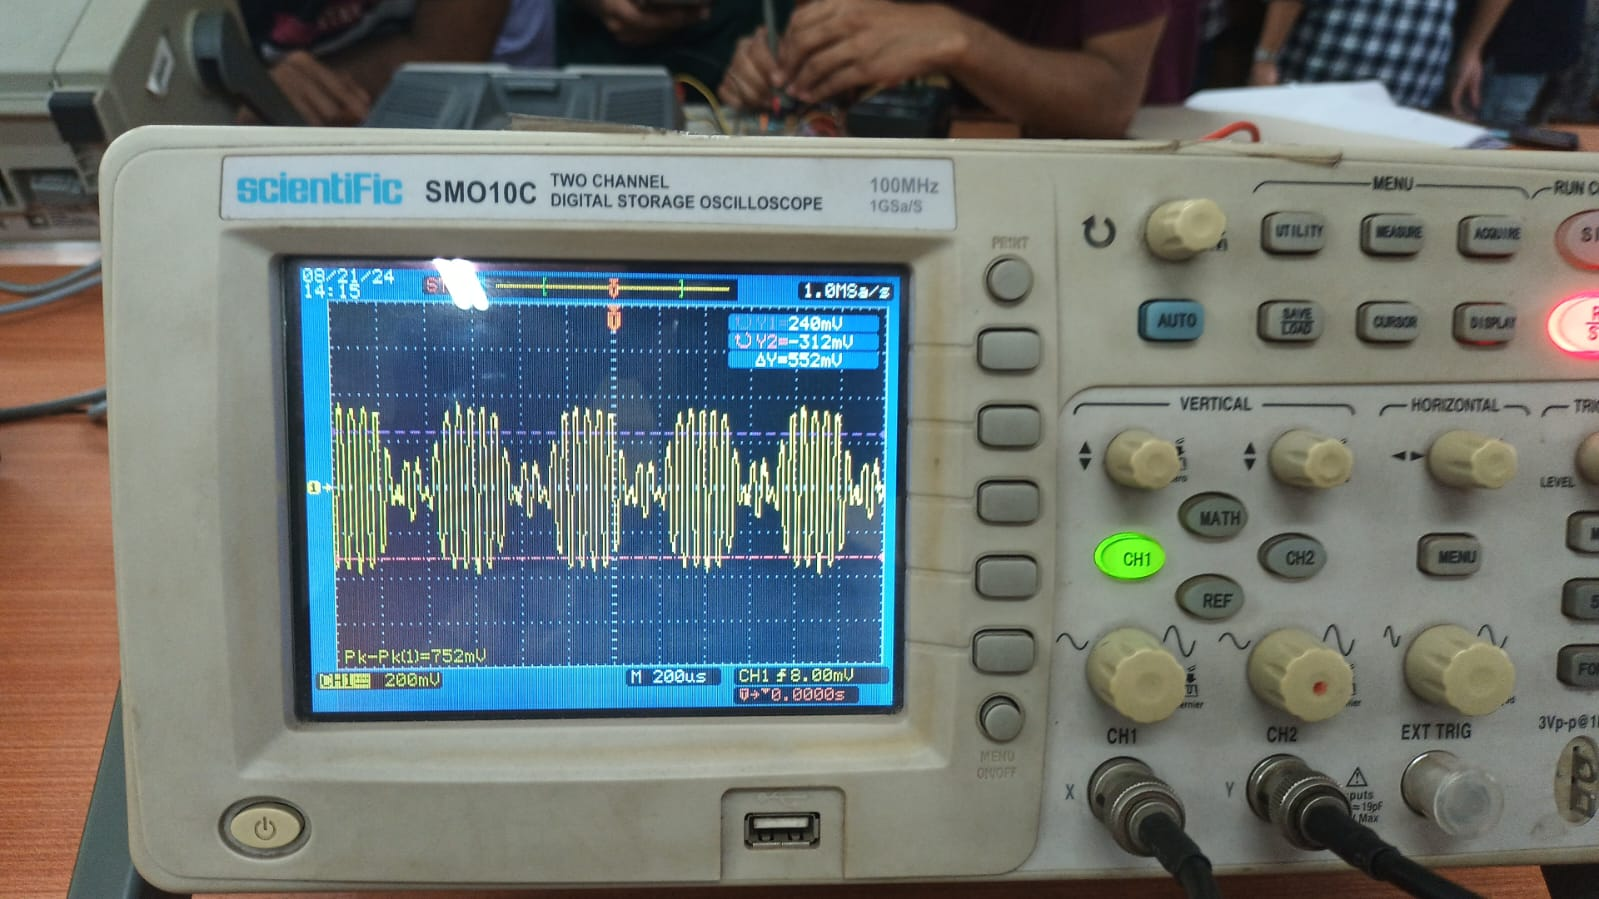
\includegraphics[width=\textwidth]{Overmodulation.jpeg}
\label{fig:Overmodulation}
\end{figure}
\begin{figure}[!ht]
  \caption{FFT of the overmodulated o/p waveform}
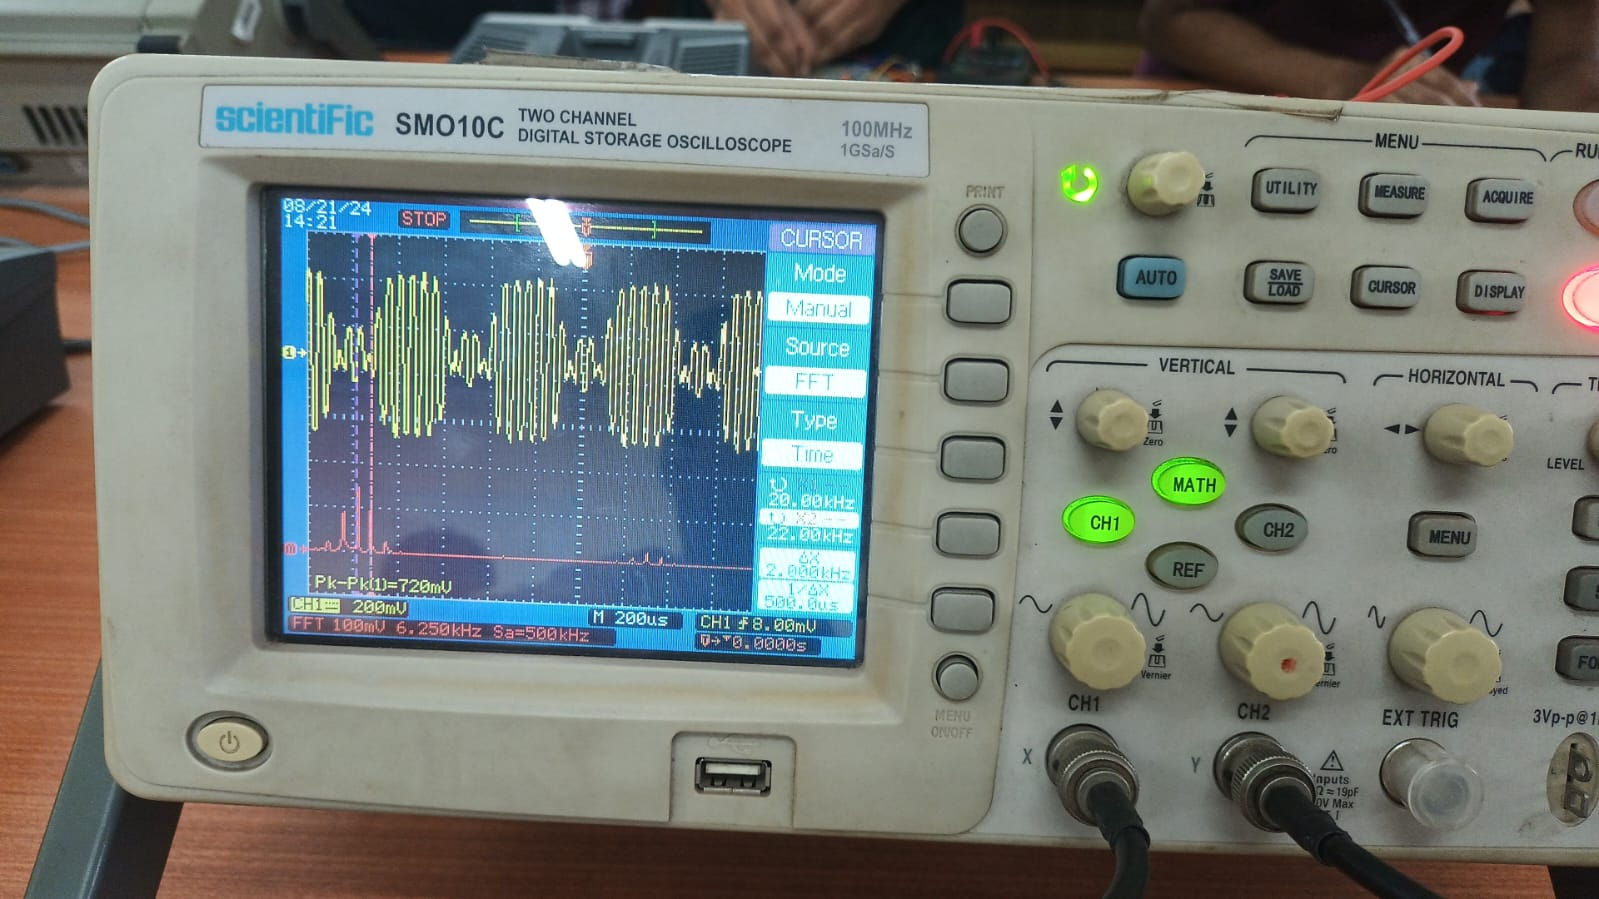
\includegraphics[width=\textwidth]{Overmodulation_FFT.jpeg}
\label{fig:Overmodulation_FFT}
\end{figure}

\clearpage
\subsection{Suppressed Carrier}
\begin{figure}[!ht]
  \caption{Suppressed carrier waveform}
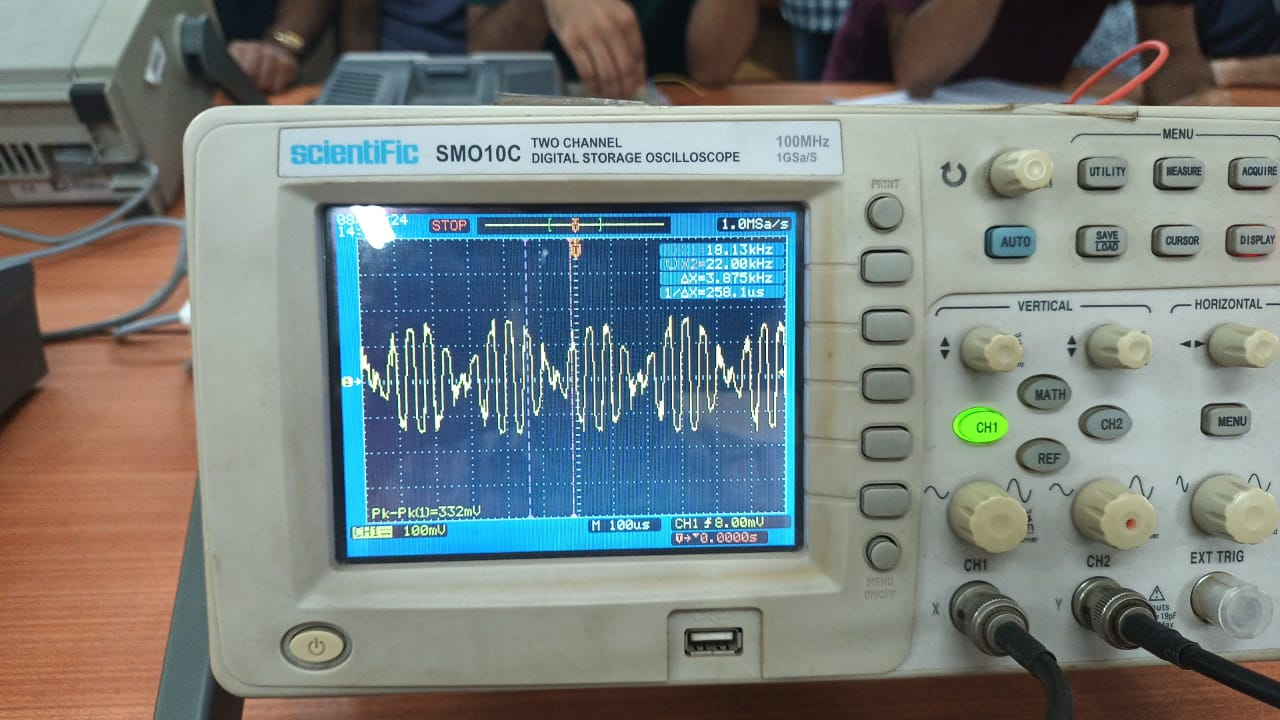
\includegraphics[width=\textwidth]{DSB_SC.jpeg}
\label{fig:DSB_SC}
\end{figure}
\begin{figure}[!ht]
  \caption{FFT of the suppressed carrier waveform}
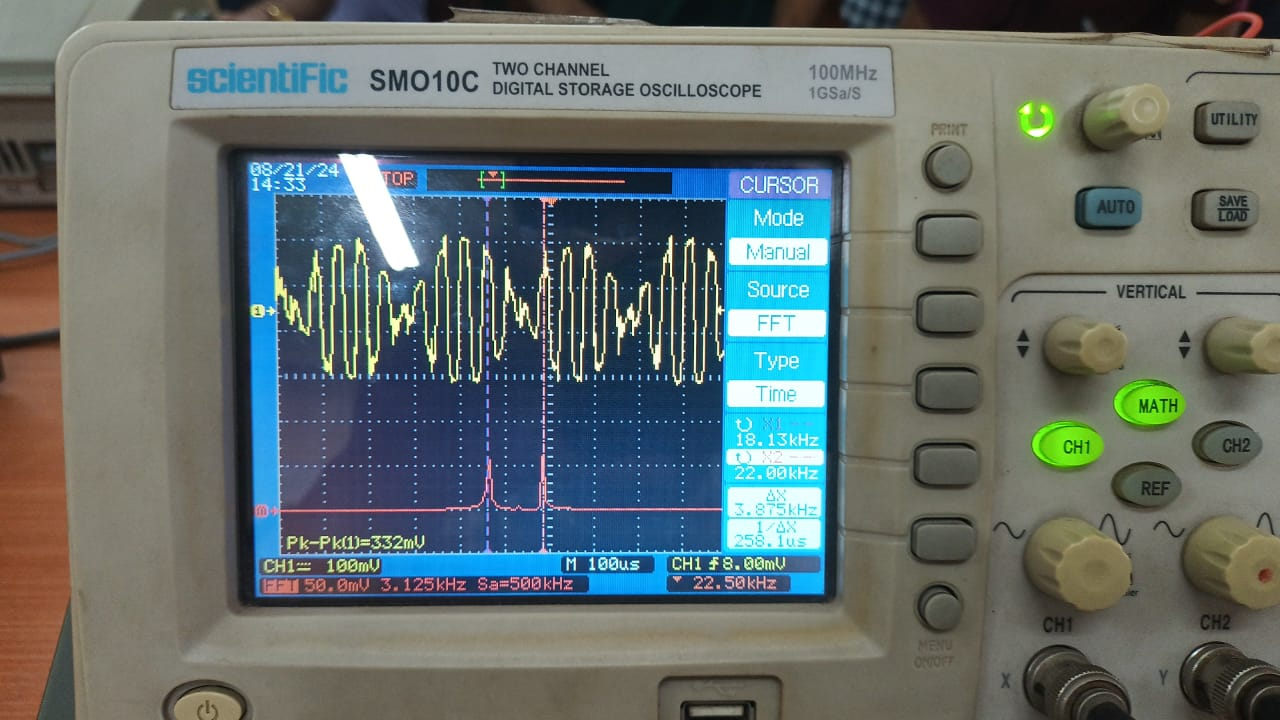
\includegraphics[width=\textwidth]{DSB_SC_FFT.jpeg}
\label{fig:DSB_SC_FFT}
\end{figure}
\clearpage
 \section{Discussion}
 \subsection{Samyak Sheersh, 22EC30045}
 \begin{enumerate}
   \item We were able to get a clearer output than the design in the previous experiment since we used an IC which would be better calibrated than our simple designs which  introduced a lot of distortions.  
   \item For each of the cases we found the following:
     \begin{enumerate}
       \item Undermodulation:
         \begin{enumerate}
           \item \emph{Time Domain}: We see that the final modulated output doesn't go all the way to zero at the minimum, and is in the same phase as the rest of the signal, as can be seen in Figure \ref{fig:Undermodulation}.
           \item \emph{Frequency domain}: We see a peak at 20kHz, and 2 much smaller peaks at 18 and 22kHz as can be seen in Figure \ref{fig:Undermodulation_FFT}
         \end{enumerate}
        \item Critical modulation:
         \begin{enumerate}
           \item \emph{Time Domain}: We see that the final modulated output goes all the way to zero at the minimum, as can be seen in Figure \ref{fig:Critical_modulation}.
           \item \emph{Frequency domain}: We see a peak at 20kHz, and 2 smaller but comparable peaks at 18 and 22kHz, and some harmonics at around 60kHz, as can be seen in Figure \ref{fig:Critical_modulation_FFT}
         \end{enumerate}
        \item Overmodulation:
         \begin{enumerate}
           \item \emph{Time Domain}: We see that the final modulated output goes back up in the opposite phase as the rest of the signal for some period, as can be seen in Figure \ref{fig:Overmodulation}.
           \item \emph{Frequency domain}: We see a peak at 20kHz, and 2 smaller but comparable peaks at 18 and 22kHz, and some harmonics at around 60kHz, as can be seen in Figure \ref{fig:Overmodulation_FFT}
         \end{enumerate}
        \item Suppressed Carrier:
         \begin{enumerate}
           \item \emph{Time Domain}: We see that the final modulated output goes all the way to zero at the minimum. It also follows a beat pattern of frequency 4kHz, as can be seen in Figure \ref{fig:DSB_SC}.
           \item \emph{Frequency domain}: We see that the carrier signal's frequency (20kHz) has been totally suppressed and does not show up in the FFT and just the frequencies of 18kHz and 22kHz remain,as can be seen in Figure \ref{fig:DSB_SC_FFT}
        \end{enumerate}
     \end{enumerate}
      \item We found the suppressed carrier signal appears only when the potentiometer is perfectly balanced. This is because perfect balancing on both sides of the differential stage doesn't provide any DC offset. 
 \end{enumerate}
\end{document}
%
